\newpage

% Table Header Box matching Page -2- of NPU form
\noindent
\begin{tabularx}{\textwidth}{|p{3.0cm}|X|X|X|X|}
\hline
\centering \textbf{\zhfont 论文题目} \newline \textbf{Dissertation Title} & 
\multicolumn{4}{p{\dimexpr\textwidth-3.0cm-4\tabcolsep-3\arrayrulewidth\relax}|}{\raggedright \textbf{Morphologically-Grounded AI-Generated Text Detection and Factual Verification for Low-Resource Agglutinative Languages: A Comprehensive Framework for Kazakh}} \\
\hline
\centering \textbf{\zhfont 论文类型} \newline {\zhfont\footnotesize (在有关项目下作记号$\surd$)} \newline \textbf{Dissertation Type} \newline {\footnotesize (Put a tick $\surd$ under relevant item)} &
\centering {\zhfont 基础研究} \newline {\footnotesize Fundamental Research} &
\centering {\zhfont 应用研究} \newline {\footnotesize Application Research} \newline \textbf{\Large $\surd$} &
\centering {\zhfont 工程技术} \newline {\footnotesize Engineering Technology} &
\centering {\zhfont 跨学科研究} \newline {\footnotesize Research Cross Discipline} \tabularnewline
\hline
\multicolumn{5}{|p{\dimexpr\textwidth-2\tabcolsep-2\arrayrulewidth\relax}|}{
{\zhfont 研究生在进行选题报告、听取意见后，整理成文（不少于 3500 字）。} \newline
\textbf{After the report and comments, make the records up to an article. (no less than 3500 words)}
} \\
\hline
\end{tabularx}

\vspace{0.6cm}

\section{Research Background}
\label{sec:background}

\subsection{Relevance and Context}
\label{sec:relevance_and_context}

The rapid evolution and widespread deployment of autoregressive Large Language Models (LLMs)---such as OpenAI's GPT-4, Meta's LLaMA-3, DeepSeek-R1, and multilingual open foundation architectures including Cohere's Aya---have fundamentally transformed artificial intelligence, automated reasoning, and natural language communication \cite{vaswani2017attention, achiam2023gpt4, dubey2024llama3, guo2025deepseekr1, ustun-etal-2024-aya}. These foundation models demonstrate exceptional proficiency in generating syntactically coherent, stylistically diverse, and contextually fluent texts across numerous domain contexts. However, the universal accessibility of advanced generative models has simultaneously escalated severe risks concerning information integrity, epistemic credibility, and digital safety \cite{bender2021stochasticparrots, solaiman2019release}. Contemporary digital ecosystems face increasing exposure to synthetic text artifacts, ranging from automated disinformation campaigns and fraudulent consumer reviews to AI-assisted academic plagiarism and hallucinated pseudo-factual assertions delivered with unmerited confidence.

Consequently, establishing robust computational mechanisms for auditing digital text content has emerged as an imperative requirement for trustworthy artificial intelligence. Reliable information verification demands two foundational capabilities: (1) \textit{AI-generated text detection}, which identifies generative origin by discerning whether a candidate text was composed by a human or synthesized by an autoregressive neural network; and (2) \textit{automated fact verification}, which evaluates whether factual propositions are substantiated by reputable reference evidence.

While extensive research has advanced text auditing in high-resource, typologically analytic or mildly fusional languages such as English and Standard Mandarin, existing methods encounter fundamental performance bottlenecks when deployed in low-resource, morphologically complex agglutinative languages \cite{khurana2024subwords, togmanov-etal-2025-kazmmlu}. Languages of the Turkic family---exemplified by Kazakh, which serves as the official state language of Kazakhstan and is spoken by over 15 million people across Central Asia---possess typological structures that directly challenge standard deep learning assumptions. In agglutinative linguistic systems, lexical roots serve as anchors for extensive, sequential suffixation chains that encode negation, syntactic case relations, tense, evidentiality, possessive markers, and pragmatic moods within single polymorphemic words. A solitary verbal root can produce hundreds of distinct surface wordforms without introducing new lexical headwords.

The proliferation of multilingual generative models within Central Asian educational, administrative, and public communication ecosystems underscores an urgent sovereign need for language-native text verification infrastructure. Without specialized auditing tools tailored to the morphological properties of Kazakh, regional media environments remain acutely vulnerable to synthetic manipulation. Developing linguistically grounded detection and verification frameworks is therefore essential for ensuring information security and linguistic equity.

\subsection{Challenges of Existing AI Detection Systems}
\label{sec:challenges_existing}

Despite substantial progress in machine-generated text detection, contemporary detection paradigms exhibit critical vulnerabilities when applied to Kazakh and typologically similar agglutinative languages:

\begin{enumerate}[leftmargin=*, label=(\arabic*)]
    \item \textbf{Subword Tokenization Fragmentation:} Prevailing transformer architectures rely on statistical subword algorithms, such as Byte-Pair Encoding (BPE), WordPiece, or SentencePiece \cite{khurana2024subwords}. These algorithms are predominantly trained on high-resource multilingual corpora, optimizing vocabulary merge operations based purely on surface frequency rather than grammatical structure. In agglutinative languages, standard tokenizers aggressively partition polymorphemic words across arbitrary character boundaries, fragmenting functional affixes into meaningless byte sequences. As illustrated in Figure~\ref{fig:fst_fragmentation}, the Kazakh word \textit{мектебіміздегілерден} (``from those who are in our school'') contains a transparent grammatical sequence of root, possessive, locative, adjectivizer, plural, and ablative morphemes. Standard subword tokenizers partition this single word into disjoint subword fragments, obscuring both the root lemma and the inflectional markers. This fragmentation inflates effective sequence lengths, depletes transformer context windows, and attenuates gradient propagation during representation learning.
    
    \item \textbf{Absence of Morphological Priors and Linguistic Grounding:} Conventional neural detectors treat text as unconstrained surface token sequences, lacking explicit inductive biases regarding root-affix compositionality, vowel harmony (palatal and labial harmony), and morphotactic suffix ordering \cite{khoshhal2020kazakh, tyers2012free}. As a result, neural classifiers struggle to distinguish natural inflectional richness from synthetic generation artifacts, frequently misclassifying formal, highly inflected human prose as machine-generated text.
    
    \item \textbf{Severe Cross-Generator and Out-of-Domain Degradation:} Zero-shot probability curvature methods (such as DetectGPT \cite{mitchell2023detectgpt}, Binoculars \cite{hans2024binoculars}, and Fast-DetectGPT \cite{bao2024fastdetectgpt}) depend on surrogate language models to evaluate local log-likelihood curvatures. In low-resource agglutinative languages, available surrogate models possess undertrained parametric vocabularies, resulting in unstable log-probability surfaces that destroy the detection signal. Supervised neural classifiers, meanwhile, overfit to generator-specific surface regularities \cite{wang2024raid, khurana2023contrastive}. When evaluated across unseen foundation model architectures (e.g., training on Sherkala-7B and testing on Qwen-2.5-7B-Instruct) or cross-domain distributions (e.g., news versus customer reviews), standard detectors experience catastrophic drops exceeding 30 percentage points in AUROC.
    
    \item \textbf{Inability to Handle Localized Synthetic Tampering:} Conventional document detectors employ uniform sequence truncation (e.g., the first 512 tokens) or naive average pooling, assuming that documents are entirely human-written or entirely synthetic. In real-world dissemination, deceptive texts are frequently created by splicing isolated synthetic sentences into authentic human articles. Naive global pooling dilutes localized forensic signals, leaving standard architectures incapable of detecting boundary-spanning hybrid manipulations.
\end{enumerate}

\begin{figure}[htbp]
\centering
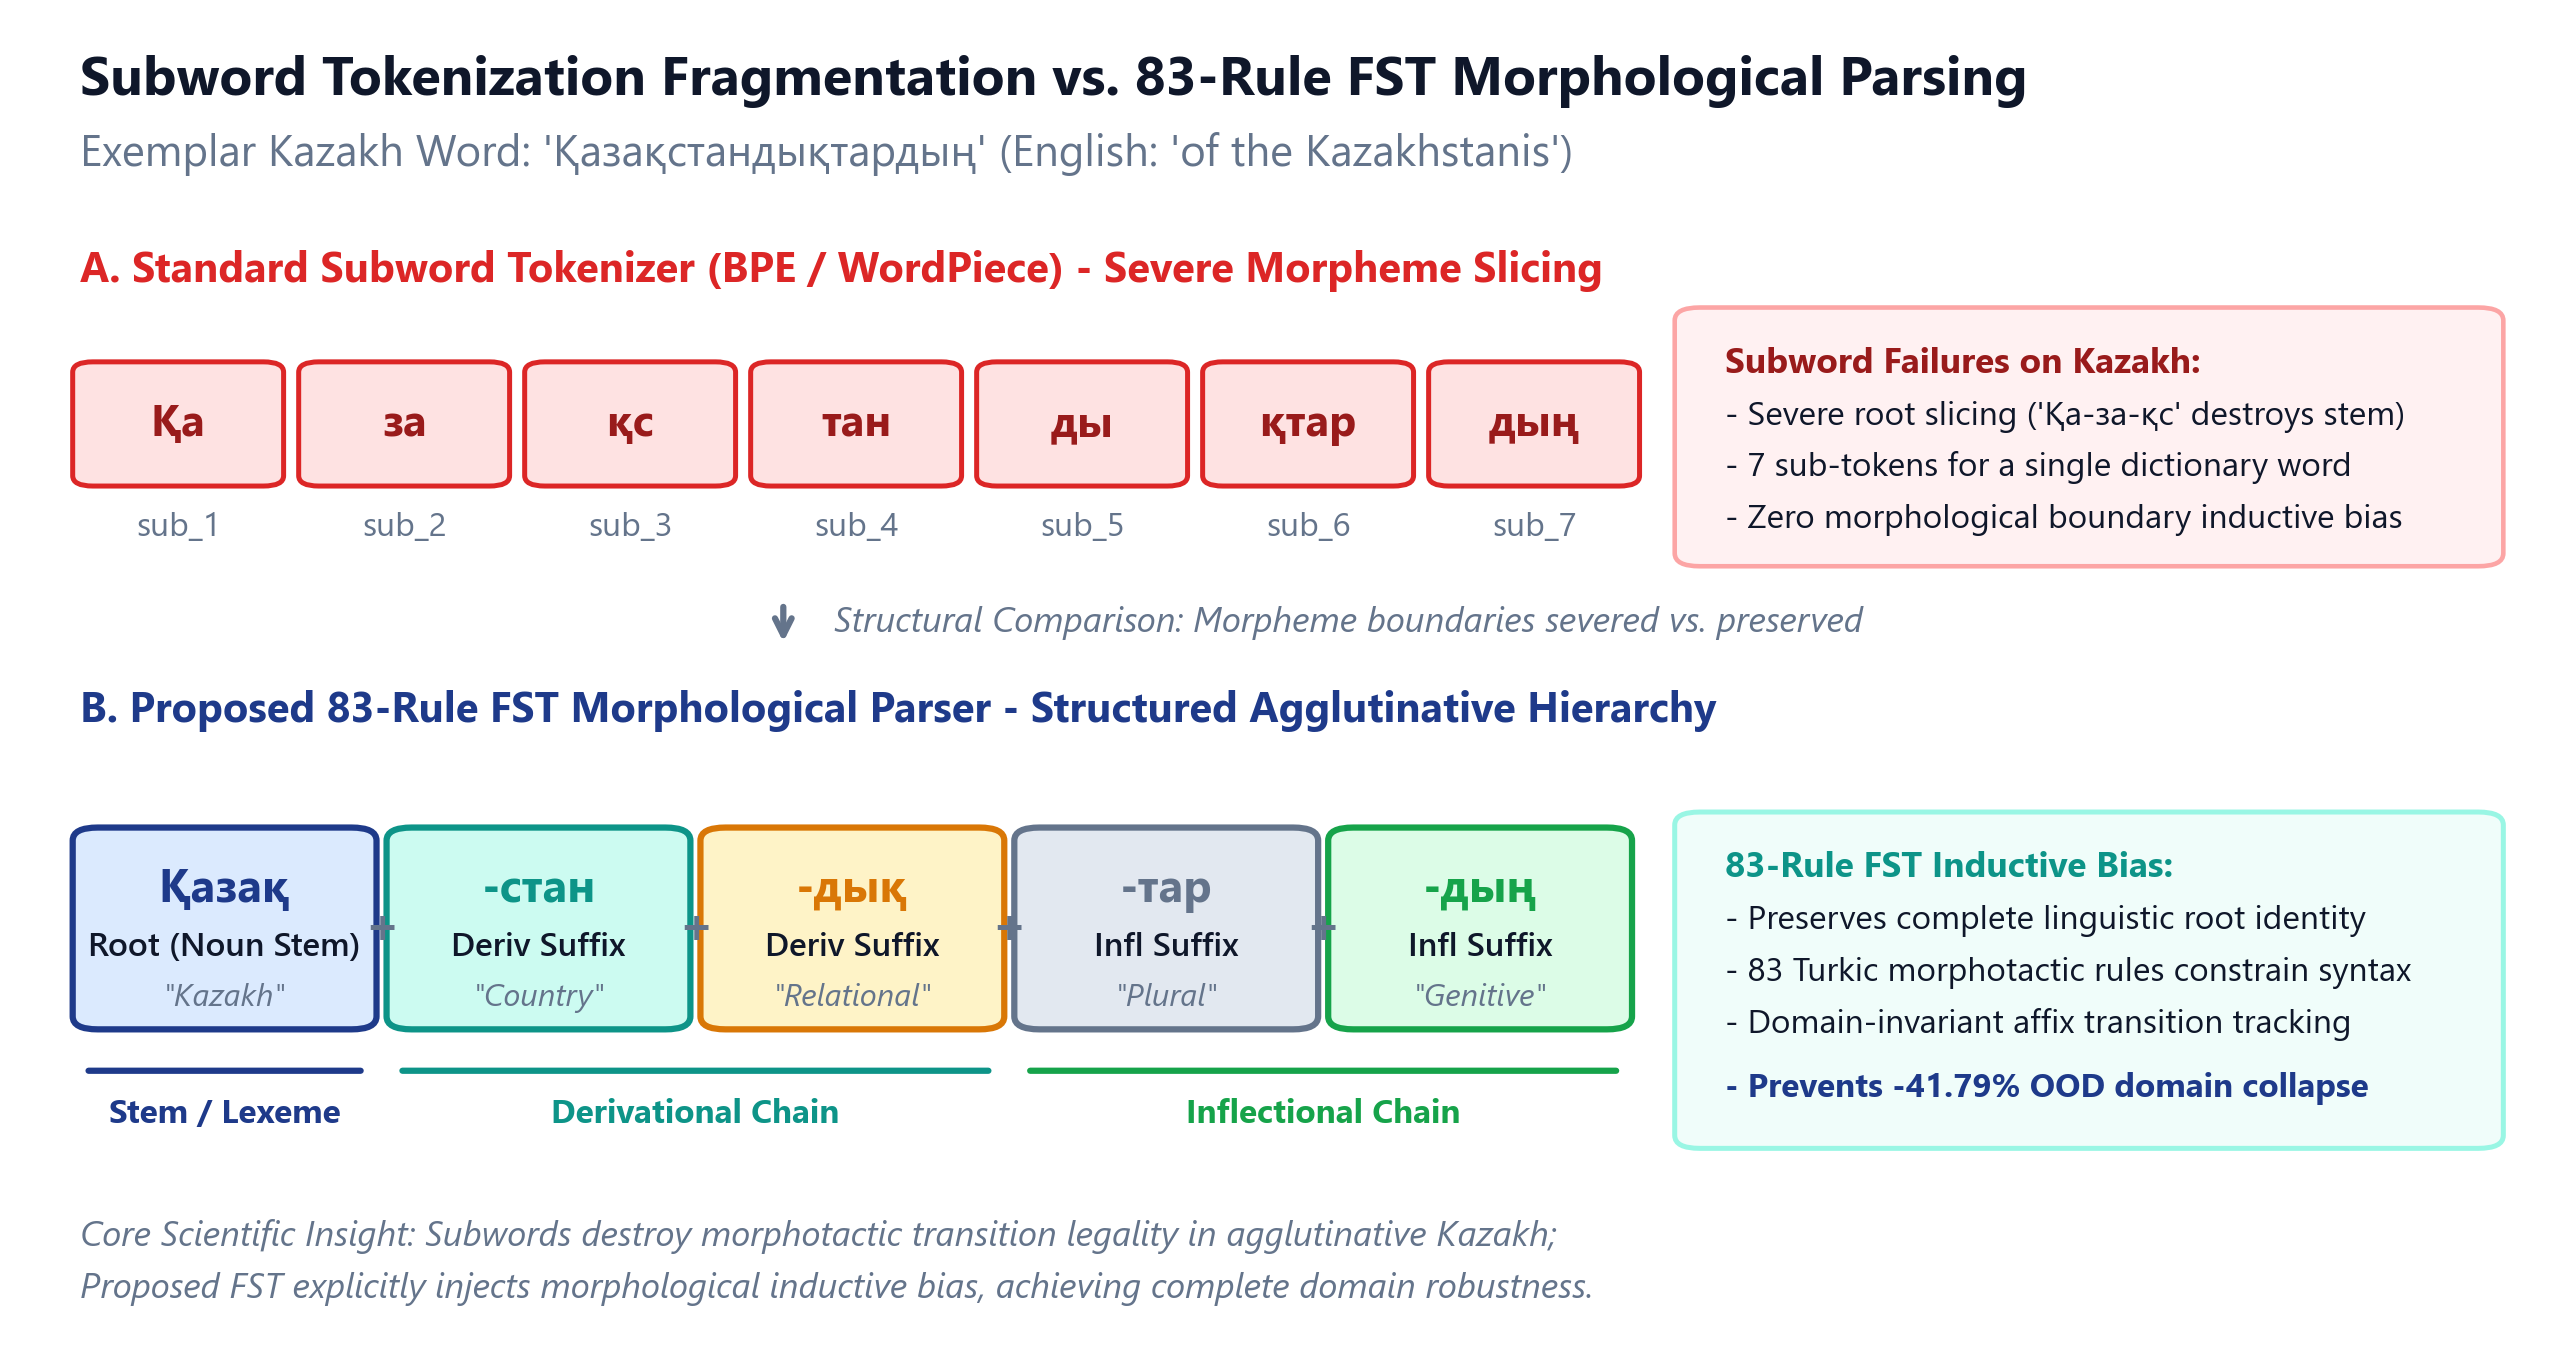
\includegraphics[width=0.92\textwidth]{figures/fig1_fst_fragmentation.png}
\caption{Subword Tokenization Fragmentation vs. 83-Rule FST Morphological Parsing in Kazakh.}
\label{fig:fst_fragmentation}
\end{figure}

\subsection{Potential of Morphologically-Grounded AI and Verification}
\label{sec:potential_morpho_verification}

To overcome the architectural and typological limitations of existing detection systems, this research proposes a morphologically-grounded computational framework that unifies symbolic morphological modeling, deep transformer representations, and multi-stage factual verification.

First, integrating formal computational morphology via an 83-rule Finite-State Transducer (FST) provides precise, bidirectional decomposition of complex agglutinative words into their canonical roots and structured inflectional tags \cite{khoshhal2020kazakh, tyers2012free}. Unlike statistical subword tokenizers that fragment words arbitrarily, the 83-rule FST explicitly models Kazakh vowel harmony, consonant assimilation, and morphotactic constraints. By coupling this symbolic morphological analyzer with pretrained deep contextual representations (such as Kaz-RoBERTa \cite{sagyndyk2025kazroberta}), our framework establishes a dual-stream architecture wherein symbolic linguistic priors directly guide neural feature extraction. This hybrid formulation neutralizes subword fragmentation, stabilizes gradient propagation, and substantially bolsters cross-generator generalization.

Second, this research recognizes that comprehensive text safety requires decoupling \textit{generative origin} from \textit{factual veracity}. In real-world media environments, machine-generated texts can articulate verified truths (e.g., automated sports or meteorological summaries), while human-authored text may propagate deliberate disinformation or rumors. Conversely, synthetic prose can hallucinate falsehoods, and human writing can record factual reality. Existing systems operate in isolated silos, failing to provide unified assessments. By introducing the first specialized Kazakh fact verification benchmark (\textbf{Kazakh-FEVER 3K}) and formulating a continuous 2D Cartesian Trust Matrix $(T_{\text{fact}}, T_{\text{gen}})$, this research establishes an interpretable, multidimensional verification paradigm that equips human fact-checkers with integrated provenance and veracity diagnostics.
